\chapter{Decision Trees}
\label{ch:bg-decision-trees}

Decision trees are one of the most important and successful algorithms
in machine learning. They have seen widespread adoption in practically
every area of machine learning, from their original domain in classification
and regression, to ranking~\cite{lambdarank}, semi-supervised learning~\cite{semi-super-trees}, survival analysis~\cite{survival-forests},
quantile regression~\cite{meinshausen2006quantile}, and unsupervised learning~\cite{tree-clustering}. In this chapter
we will provide a brief review of the literature on decision trees in
areas that are relevant to our work, namely ensembles of decision
trees and online decision trees. For a comprehensive review of
decision tree literature we refer the reader to the monograph
by \citet{decision-trees-book} or the extended survey by \citet{tree-survey}.

\section{Learning Algorithms}
\label{sec:bg-dt-learning-algorithms}

The two original tree-learning algorithms, the
Classification and Regression Trees (CART)~\cite{breiman1984cart} algorithm and the ID3
algorithm~\cite{id3}, were developed in parallel. In our description we will
focus on the CART regression algorithm, following the description from \cite{esl}.

Decision trees create recursive binary partitions of the input space,
with axis parallel cuts. Let $R_1, ..., R_M$ denote the $M$ regions created by
the model.
The model predicts the same value $\hat{c}_m$ for all data points
that fall under the same region in the partitioned space. For regression,
using the sum of squared errors as the objective function, the best possible
$\hat{c}_m$ is the average of the label values in that region.
Finding the optimal partitioning for decision trees is known to be
NP-complete \cite{dt-np-complete} and the best possible method
is to use a greedy algorithm to select the splits~\cite{dt-hardness}.
In the regression case, CART achieves that by selecting splits
that minimize the squared error of the created binary split, selecting
for each region the average value of the labels.
In the classification case, the splitting criterion is an information-theoretic
node impurity measure like the Gini index or the cross-entropy, defined as:

\begin{equation}
	\begin{split}
		\text{Gini Index} = \sum_{k=1}^K\hat{p}_{mk}(1 - \hat{p}_{mk}), \\
		\text{Cross-entropy} = -\sum_{k=1}^K\hat{p}_{mk} \log{\hat{p}_{mk}},
	\end{split}
\end{equation}

\noindent
where $k$ the class, $m$ the node and $\hat{p}_{mk}$ the proportion of
the observations for class $k$ in the node $m$.

While one could keep growing a decision tree until it perfectly fits the data,
that will lead to overfitting and bad generalization. Therefore
it is common to employ some form of \emph{pruning} strategy to limit the
complexity of the model. This can be done by introducing some
form of complexity penalty to the tree, limiting the number of terminal
nodes, or having a minimum number of examples in each terminal node
\cite{breiman1984cart}. This process is also important in limited
memory settings where deleting and merging nodes can lead to models
that take up less space in memory, especially in ensemble approaches
mentioned in the sequel. A creative approach to reducing model size are decision
jungles that change the data structure being learned from a tree to DAG, allowing
nodes in a the tree to have more than one parent,
providing the same learning capability using fewer nodes~\cite{decision-jungles}.


\section{Ensembles of Decision Trees}
\label{sec:bg-dt-ensembles}

The success and popularity of decision trees comes in large part
from their use in model ensembles.
As mentioned in Section \ref{sec:bg-ol-ensembles}, the two dominant paradigms in ensemble learning are \emph{bagging} \cite{bagging} and
\emph{boosting} \cite{boosting-schapire, boosting-freund-schapire}. Both
methods can be interpreted using a resampling procedure. Bagging is
based on the bootstrap \cite{bootstrap} resampling method and will re-use samples
to train the members of the ensemble, and average their predictions.
% Bagging can be used to reduce both the bias and variance of a learning method.
Boosting methods on the other hand will assign increased weights to the
hardest instances in the data. In the ``AdaBoost.M1'' version of the algorithm,
a new weak learner is trained at each iteration, and a weighted sum of
the decisions of each learner is taken to produce the final prediction.
Further work by \citet{gradient-boosting-breiman} established a statistical framework
for boosting and formalized \emph{gradient boosting} as gradient descent in function
space.

Decision trees have been used as parts of either bagging
or boosting ensembles with great success~\cite{hundreds-classifiers}. Their characteristics as a fast
non-linear learner
with high flexibility fit well both the bagging and boosting paradigms.
The \emph{random forest} algorithm uses bagging to train an ensemble
of randomized trees and combine their predictions, while gradient boosted trees
uses a combination of trees and gradient boosting to produce
accurate learners. In the following we give a brief overview for each method,
and refer the reader to \cite{random-forest-survey, tree-survey} and \cite{biau-optimization} for recent surveys on
random forests and gradient boosting respectively, or the introductory monograph by \citet{esl}.

\subsection{Random Forests}
\label{sec:bg-dt-random-forests}

Random Forests (RF), originally proposed by \citet{random-forests}, have been shown to be one of the
most versatile algorithms in machine learning~\cite{hundreds-classifiers}. They are an
ensemble method the combines multiple randomized trees, each trained with a sample
of the original dataset, and averages their predictions to produce the final outcome.
Random forests can deal with classification or regression tasks and provide estimates
of the importance of variables, aiding in their interpretability.

Following the notation in \cite{random-forest-survey}, the algorithm works by growing
$M$ randomized trees, each on a sample from the original dataset $a_n$. The sample
$a_n$ can be taken with or without replacement, although usually it is a boostrap
sample~\cite{bootstrap} with a size equal to the original dataset. In the original
algorithm by \citeauthor{random-forests}, the trees are grown using the CART criteria,
with the difference that we limit the number of features being
considered for the splits, with \citeauthor{random-forests} selecting one feature or
$log_2{p} + 1$, while \citeauthor{random-forest-survey} recommend using $\lceil p/3 \rceil$;
see \cite{rf-parameters} for an investigation of RF parameter settings.
For the regression task the predictions of the forests are calculated
by taking the average prediction of all trees, while for classification
we take a majority vote among all trees.

The random sampling and independent growing of each tree provides two distinct advantages
to the RF algorithm. First, because the trees are grown independently, unlike the boosted trees
discussed in the next section, parallelizing their learning is trivial. In the parallel
setting where we have access to the complete dataset, or if the complete dataset
fits in memory, parallelization is as simple as training a different tree on
each bootstrap sample. The situation changes
however for distributed data because of the nature of the bootstrap: depending
on the sample selection there might be the need for data points to be communicated
over the network, with a resulting high communication cost.
\citet{ensembles-bites} propose instead to train the trees independently
and merge the votes, or one could make use of the bag of little bootstraps
to train the models \cite{bag-of-boostraps}. Alternatively, we can create split
histograms on data partitions and communicate those over the cluster to determine the
best split for each leaf, similar to how trees are grown for distributed
gradient boosted tree methods~\cite{xgboost, lightgbm}.

Second, the fact that for each tree some samples from the dataset are not
used to train it, known as \emph{out-of-bag} (OoB) samples, creates opportunities
to use those data points to extract useful information about the performance
of the tree. We can use the OoB samples to adjust the hyper-parameters of the
algorithm without the need to use a validation dataset. We can also use
the out-of-bag sample to estimate \emph{variable importance}.
\citet{random-forests} proposed the Mean Decrease Accuracy measure of
variable importance, where using the OoB instances for a tree, we
randomly permute the values a feature, and make predictions
for the permuted and original data. We take the average
of the difference of the OoB error between the permuted
and original data and use that as an estimate of the importance
of the variable. \citet{random-forest-survey} note that this approach has issues with correlated variables, because the
algorithm tests variables in isolation rather than conditional
to each other.
Finally, \citet{johansson2013conformal} make use of the OoB samples to provide
uncertainty estimates in inductive conformal prediction, without the need for a
validation set, a property we exploit in \uncertaintrees as well.

\subsection{Gradient Boosted Trees}
\label{sec:bg-dt-gbts}

Gradient boosted trees have risen to be one of the most popular algorithms
in machine learning due to their speed, scalability, and accuracy. Efficient
implementations like XGBoost \cite{xgboost} and LightGBM \cite{lightgbm}
are now widely deployed in production use-cases, and further emphasis
is being given to efficient training \cite{dimboost} and inference \cite{quickscorer, tree-cache-conscious, tree-runtime-opt}.
In this section we will describe the training and prediction process of GBTs,
with a focus on the scalability aspect of the algorithm. We provide an in-depth
description of the histogram construction algorithm which we have found to be missing
from most relevant literature. We refer the interested reader to a recent overview
of the optimization process of GBTs by \citet{biau-optimization}.

\subsubsection*{Model}

The gradient boosted tree model consists of an ensemble of decision trees,
which are trained in an additive manner. At each iteration a new tree is added
to the ensemble, chosen so that it minimizes an objective function.

We use the
regularized objective formulation used
in \cite{xgboost}, and follow their notation throughout our description of the algorithm.
The objective function is shown in Eq. \ref{eq:gbt-objective}

\begin{equation}
	\begin{split}
	\mathcal{L}(\phi) = \sum_{i} l\left(\hat{y}_{i},y_{i}\right) + \sum_{k} \Omega\left(f_{k}\right) \\
	\text{where } \Omega\left(f_{k}\right) = \gamma T + \frac{1}{2} \lambda \norm{w}^2
	\end{split}
	\label{eq:gbt-objective}
\end{equation}

\noindent
where $l(\cdot, \cdot)$ is a differentiable loss function and $\Omega$ is a regularization term
that penalizes complex models. The regularization term takes into consideration
the number of leaves $T$ and the norm of the weights at the leaves $w$. This helps
smooth the weights to avoid overfitting. This objective defined in XGBoost
has then been used in follow-up GBT learning systems like LightGBM and
DimBoost \cite{lightgbm, dimboost}.  A note here is that XGBoost
assumes that the loss function is twice differentiable in order
to calculate the Hessian analytically for each loss function.
However, as shown recently in \cite{accelerated-gb} it is possible
to use Nesterov's first-order accelerated gradient descent method
\cite{nesterov-book} to produce gradient boosting models of similar
accuracy, while being much more sparse in the number of components.
In distributed training this would have the added benefit of reducing
the amount of data being communicated by half, as we would only need to
communicate first-order gradients and not Hessians, as we explain
in the following section.



\subsubsection*{Training}

\begin{table}
	\centering
	\begin{tabular}{cccc|c}
		\toprule
		Index & Feature 1 & Feature 2 & Feature 3 & Gradient \\
		\midrule
		\rowcolor{CBOne}
		1 & 13 & 0 & 488 & 1.5 \\
		\rowcolor{CBTwo}
		2 & 7 & 1 & 667 & 2.5 \\
		\rowcolor{CBThree}
		3 & 3.5 & 0 & 122 & 2 \\
		\rowcolor{CBFour}
		4 & 1.6 & 2 & 366 & 2.5 \\
		\bottomrule
	\end{tabular}
	\caption{Example dataset.}
	\label{tab:example-data}
\end{table}


The training process for a single gradient boosted tree can be roughly divided into three stages:
First, we use the existing ensemble to make predictions for every data point in the training
set. Second, we use the approximated objective function to determine the first and second order
gradients for each data point. Finally, we use the calculated gradients to greedily determine
the optimal split for every leaf in the tree. When we mention gradients here we are referring
to both the first order and second order gradients for $x_i$, denoted as $g_i$ and $h_i$
respectively.

We will focus on the third part of the training stage in our description, as that entails the most
computationally intensive part of GBT learning, the construction of the \emph{gradient histograms.}
Throughout our examples we'll be using the dataset from Table \ref{tab:example-data},
which we color-code by instance to correspond to the figures used later on.

As a tree grows, we partition the complete training set into smaller parts, with each data
point ending up in one leaf as we drop it down the tree.
In order to determine the best split for every leaf, we need to iterate through the data
partition of each leaf and create a gradient histogram for each feature for that leaf.

In its simplest form, a gradient histogram gives us the sum of gradients at a leaf,
given a feature value, that is, $\sum_{j}(G_i | x_i(f) = f_j)$, where $x_i$ is a data point
that belongs to the current leaf,  $G_i$ is the gradient value of $x_i$ and $j$ is an
indicator over the unique values of the feature $f$. In other words, it gives us the
sum of the gradients of all data points in the leaf for a specific value of a given
feature $f$.

Enumerating every gradient-feature value combination requires that we calculate
a gradient sum for each unique value
of a feature. This can quickly become computationally impractical for real-valued features, as we might have millions or billion unique feature values.
Systems like XGBoost and LightGBM instead use \emph{quantized histograms},
where we accumulate gradients for ranges of values in histogram buckets for every feature.

To determine the bucket ranges we
can use \emph{quantile sketches} \cite{greenwald2016quantiles} that approximate
the Cumulative Distribution Function (CDF) of each feature. We select a number of
equi-weight buckets, that is, the ranges are selected such that every bucket
has approximately the same weight-sum of data points. In the simplest case
all instances have the same weight, and regular quantile sketch algorithms
can be used, otherwise specialized, weighted sketches like the ones used by XGBoost
have to be employed.
The number of buckets to use is a
parameter of the quantile sketch algorithm and depends on the type of sketch.
There exist sketches where we select the number of buckets that
will be used to represent the CDF, like the ones proposed by \citet{BenHaim2010parallel}
or the number of buckets is derived from the approximation error we choose for the sketches, for example
for the sketches used by XGBoost or by the state-of-the-art KLL sketch \cite{karnin2016kll}
used by DimBoost \cite{dimboost} and in our own work in Papers \uncertaintreesNum and \blockgbtNum.

\begin{figure}
	\centering
	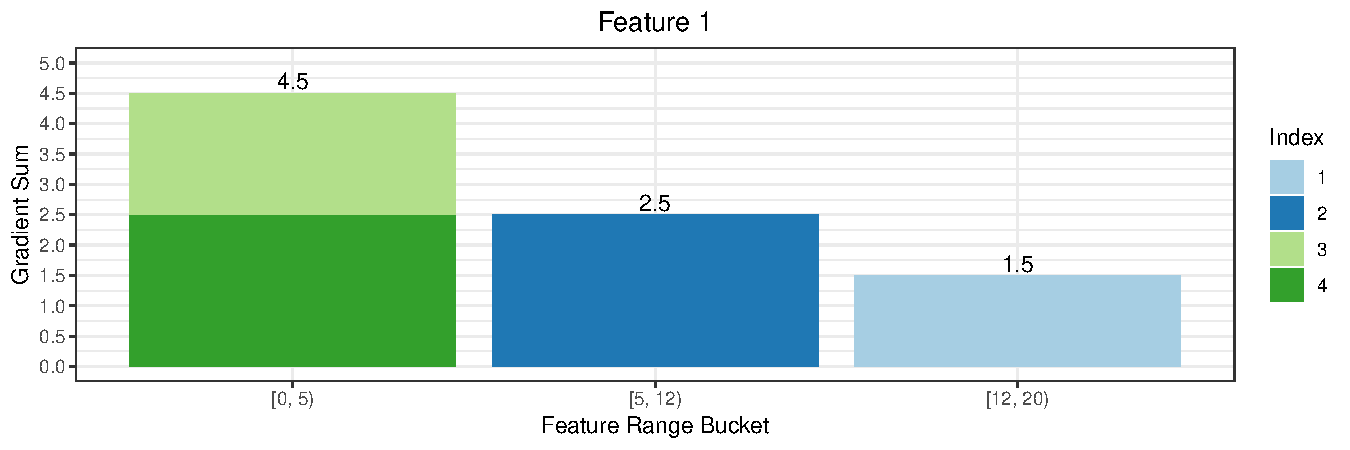
\includegraphics[width=\columnwidth]{feature-one-grad}
	\caption{Gradient histogram for Feature 1 of the Table \ref{tab:example-data} data.
	The first bucket is the sum of the data points with index 3 and 4, since both their Feature 1
	values fall in the $[0, 5)$ bucket.}
	\label{fig:gradient-feature-one}
\end{figure}


The selection of bucket ranges can be done either at the beginning of training, taking the
overall feature CDF, or at every leaf taking the CDF of each feature using only the
partition for that leaf. \citet{xgboost} show that by selecting the buckets for every
leaf separately, we can achieve the same level of accuracy, while using histograms with a higher approximation error, and hence reducing the memory footprint of the algorithm.


Once the bucket ranges have been determined for each feature, we use them to create
the gradient histograms. After the prediction step, we have a gradient value for each data point, so
we go through each feature and add the data point's gradient value to the gradient
histogram bucket
that corresponds to the feature value.
In our example data in Table \ref{tab:example-data}, for Feature 1 we use the
buckets $[0, 5), (5, 12], (12, 20)$.
Then, for the data point $x_1$ with a feature value $f_1 : 13$, we would add its
gradient value to the
the bucket $(12, 20]$ of the gradient histogram for $f_1$, and do this for
every data point, adding the point's gradient to the corresponding bucket given
the feature value. The gradient histogram for Feature 1 is shown in Figure \ref{fig:gradient-feature-one}. In the Figure we use color to identify the
contribution of each data point to each bucket.
When we are done iterating, each feature will have a corresponding gradient histogram,
whose sum is equal to the sum of gradients for the leaf.
For the data of Table \ref{tab:example-data}, the complete gradient histograms
are shown in Figure \ref{fig:gradient-all-features}.

\begin{figure}
	\centering
	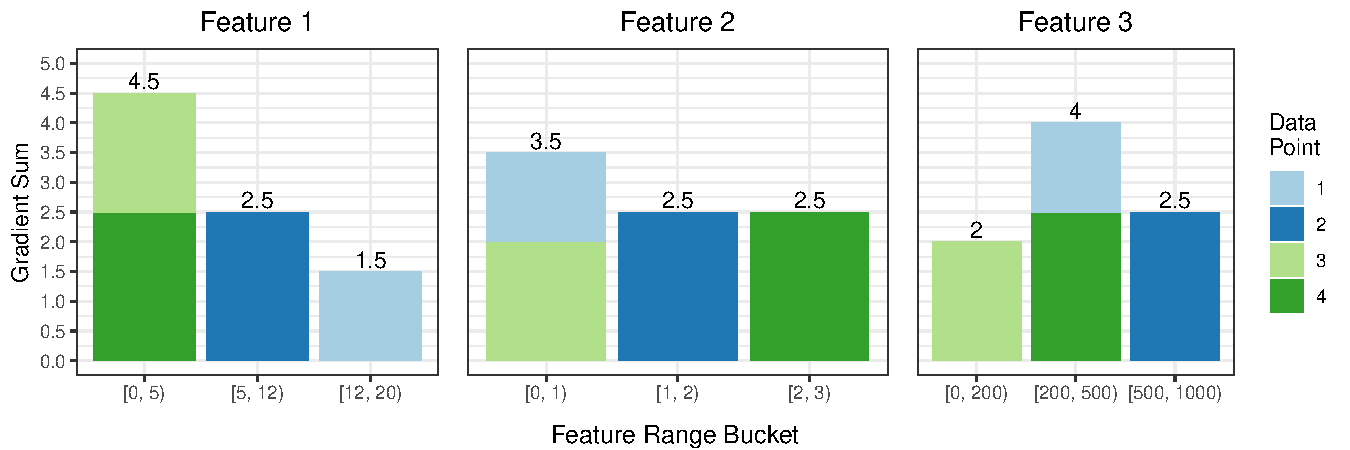
\includegraphics[width=\columnwidth]{all-features-grad-custom}
	\caption{Gradient histograms for all features of the Table \ref{tab:example-data} data.
		}
	\label{fig:gradient-all-features}
\end{figure}

Once we have all the gradient histograms, we can use them to determine the optimal split point for the
leaf, by calculating the potential gain of each feature and split point combination using the following equation~\cite{xgboost}:

\begin{equation}
	\mathcal{G}_{\text{split}} = \frac{1}{2} \left[\frac{\left(\sum_{i \in I_{L}} g_{i} \right)^{2}} {\sum_{i \in I_{L}} h_{i}+ \lambda} + \frac{\left(\sum_{i \in I_{R}} g_{i} \right)^{2}}{\sum_{i \in I_{R}} h_{i} + \lambda} - \frac{\left(\sum_{i \in I}g_{i}\right)^{2}}{\sum_{i \in I}h_{i}+\lambda}\right]-\gamma
\end{equation}

\noindent
where $I_L, I_R$ determine the data points that end up to the left and right side of the split
respectively, $I$ is the complete set of data for the leaf partition, and $\gamma$ a
regularization parameter. At this point, to determine
the best split we need to simply iterate through all the feature-splitpoint combinations
and rank every candidate according to their loss reduction (or \textit{gain}) and select the
best one. In our example we have three buckets, and hence two possible split points for each feature. The result for our example data is shown in Table \ref{tab:gains}, where
we have simplified the problem to only include the first order gradients. From that example
we can see that the best feature-split combination would be choosing the first split
point for the first feature (i.e. Feature 1 $< 5$) as the split condition.

\begin{table}
	\centering
	\begin{tabular}{ccc}
		\toprule
		& Splitpoint 1 & Splitpoint 2 \\
		\midrule
		Feature 1 & \textbf{36} & 21 \\
		Feature 2 & 35 & 30 \\
		Feature 3 & 26 & 30 \\
		\bottomrule
	\end{tabular}
	\caption{Potential gains for each possible split point, given
	the gradient histograms of Figure \ref{fig:gradient-all-features}.}
	\label{tab:gains}
\end{table}

In the case of millions of features and a large bucket count this can also be
computationally heavy operation, as we need to evaluate $|F| \times B$ split candidates.
To mitigate this, we can apply efficient boosting approaches that try
to reduce the number of features being examined. Examples include LazyBoost \cite{lazyboost}
that uniformly subsamples the set of features,
bandit methods \cite{bandits-boosting} that use information from previous iterations, or other adaptive
methods like Laminating \cite{laminating} that determines the best feature in multiple rounds, by incrementally
halving the number of features being considered and doubling the number of examples being
included in the gradient calculations.

\section{Online Decision Trees}
\label{sec:bg-dt-online-trees}

As we have shown, decision trees are trained by recursively splitting the complete
training set as we introduce more leafs. This process is incompatible with the online
learning scenario where data points arrive sequentially and we never have access to
the complete dataset. To tackle such a scenario, a number of online decision tree
alternatives have been proposed.

\subsubsection*{Hoeffding Trees}

By far the most popular online decision algorithm for classification is the Hoeffding Tree (HT) \cite{vfdt},
which has served as the basis for most of the follow up work on online decision
trees. The aim of the HT is to create an online decision tree algorithm that will converge
to its batch equivalent given enough samples.
The learning in an HT, or as \citet{vfdt} name it, the Very Fast Decision
Tree (VFDT), happens only at the leaves, and every data point is only utilized
once, i.e. the HT is a single-pass algorithm. The leaves accumulate statistics
with the purpose of probabilistically determining the best split. The tree gets its
namesake from the use of the Hoeffding bound to determine if we have accumulated
enough information at a leaf to trigger a split with high confidence.

Following the description from \citet{vfdt}, the Hoeffding bound \cite{hoeffding-bound} is a probability inequality that allows
us to probabilistically bound the true mean of a random variable $r$ for which we have
made $n$ independent observations and computed their sample mean, $\bar{r}$. Given
the range of the variable, $R$, the Hoeffding bound states that with probability
$1-\delta$, the true mean of the variable $r$ will be at least $\bar{r}-\epsilon$, where
$\epsilon$ is defined as:

\begin{equation}
	\epsilon = \sqrt{\frac{R^2ln(1/\delta)}{2n}}.
\end{equation}

In VFDT, the Hoeffding bound is used to determine with a high degree of certainty when
it is time to split a leaf. Let $G(X_i)$ be the measure used to choose the feature
to split on. As we mentioned in Section \ref{sec:bg-dt-learning-algorithms}, this can be
information theoretic measures like the cross-entropy or the Gini index. Ideally we want the feature we select given a limited sample of $n$ examples, to be the same as would be chosen given infinite examples.
The Hoeffding bound allows us to achieve that with high probability by applying
it to determine the maximum possible difference between the best and second best
features to split on. Specifically, let $\bar{G}(X_a)$ be the heuristic value for the
current best feature, after having observed $n$ instances, and $\bar{G}(X_b)$ the second
best. The difference between these two is $\Delta \bar{G} = \bar{G}(X_a) - \bar{G}(X_b)$.
We can then use the Hoeffding bound to determine that $\bar{G}(X_a)$ is indeed the
best feature to split on with probability $1-\delta$, if $\Delta \bar{G} > \epsilon$.

The process of learning at each leaf is then the following: For every incoming sample
that ends up in a leaf, we update the sufficient statistics for that leaf, which we
use to calculate the heuristic for the split, e.g. the Gini index. Theoretically,
one could check if we have gathered enough information to split a leaf after each
incoming sample, but that would introduce a large computational overhead. What we
do instead, for example in the implementation of the algorithm in the MOA library \cite{bifet2010moa},
is to only check if the Hoeffding bound is satisfied periodically, for example
every 200 samples. Another parameter of the algorithm is the probability of an error,
$\delta$. This parameter can have a large effect on the final tree, as setting it
too high can lead to early splits being taken that end up being sub-optimal, and as a result,
values in the order of $10^{-7}$ are often used \cite{data-stream-mining}.

HT was designed for the classification setting, where handling discrete attributes
is straightforward: we can just keep a table of frequencies for classes and feature
values. The situation
is different for continuous attributes however, where we need to maintain per-class
information about the values. In the worst case we would need to maintain the class
frequencies for every unique value in a continuous feature, something that is impractical
for online learning, where datasets are potentially unbounded and the memory footprint
of the algorithms should remain as small as possible. For features with many repeated
values it is possible to use a binary tree structure with counters that allows for
fast storage of the values, however this again has a large memory cost. Alternatives include
using online histograms or quantile sketches \cite{greenwald2016quantiles}
to maintain approximations of the Cumulative Distribution Function of
each feature, or approximating the distribution of each continuous feature using a Gaussian.
We refer the interested reader to Chapter 4 of \citet{data-stream-mining} for details on these methods.

The Hoeffding Tree has served as the starting point for most of the follow up work on
online decision trees. \citet{vfdt-normal} use a ``Normal'' test to improve
upon the statistical efficiency of the Hoeffding bound. The proposed method achieves
the same probabilistic bound with a reduced sample size, by taking
advantage of properties of the Gini index and entropy. More recently,
\citet{efdt} propose an algorithm that uses the Hoeffding bounds but
will re-visit nodes that have already been split and evaluate if their
split decision should be updated. This leads to a large improvement in accuracy
compared to the base HT,
at the cost of added computation and memory necessary to maintain
the sufficient statistics for internal nodes and re-evaluate split
decisions.

In a contrasting view, \citet{vfdt-mcdiarmid} claim that the assumptions made
by the Hoeffding bound-based algorithms are commonly violated as the bound assumes
real-valued data, and the fact that measures like the Gini index and information
gain cannot be expressed as sums of elements. As an alternative they propose
using McDiarmid's inequality of which Hoeffding's inequality is a special case.
Their use of the McDiarmid
bound is however computationally intensive. This drawback is mitigated
in their follow-up work \cite{vfdt-gaussian} which follows in part the work from \citet{vfdt-normal}
and provides a bound on the information gain difference between two potential
split attributes based on the Gaussian distribution.

One of the few online decision tree algorithms that is aimed at regression
is the Fast Incremental Model Tree (FIMT) algorithm by \citet{fimt}, also
based on the HT. FIMT
is a model tree, i.e. instead of simply using the average of the labels
in its leaves to make predictions, it maintains a linear model, which is
fit on the samples arriving at the leaf, and is then used for prediction.
The merit of a split is calculated based on the Standard Deviation Reduction (SDR),
similarly to batch regression trees like the M5 model \cite{m5-tree}, defined as:

\begin{equation}
	\begin{split}
		\text{SDR}(h_A)=sd(S)-\frac{|S_L|}{|S|}sd\left(S_{L}\right)-\frac{|S_R|}{|S|}sd\left(S_{R}\right), \\
		sd(S) = \sqrt{\frac{1}{|S|}\left(\sum_{i=1}^{N}y_{i}^{2}-\frac{1}{|S|}\left(\sum_{i=1}^{N}y_{i}\right)^{2}\right)}
	\end{split}
\end{equation}

\noindent
where $h_A$ is the proposed split on feature $A$, and $S_L, S_R$ the resulting
data partitions on the left and right side of the split.

SDR is possible to be calculated online, by maintaining only three statistics per leaf,
making the learning of these trees efficient. However, the base FIMT uses a binary tree
to store feature values, leading to a potentially high memory cost, for which
the authors provide solutions like disabling non-promising split points and dropping
parts of the tree. To determine the
probability of a split being optimal, the authors again use the Hoeffding bound
on the SDR ratio of the two best splits which will be in $[0, 1]$ range.
The linear models at the leaves are perceptron models, updated using stochastic
gradient descent.  Finally, FIMT includes a change detection system in order to
adapt to concept drift
based on the Page-Hinckley change detection test~\cite{ph-test, ph-test2}.

\todo{Online RFs?}

\subsubsection*{Mondrian Forests}

All the methods we mentioned so far have made use of the same base tree building
algorithm that was first proposed for VFDT: each data point is only evaluated once,
the statistics are maintained only at the leafs, with the exception of \cite{efdt},
and heuristics that take into consideration the conditional distribution of the
features given a class are used to determine the splits. \citet{mondrian-forests-original}
proposed a new class of algorithm based on Mondrian processes \cite{mondrian-process}
that provides a new way to train decision trees online.

Mondrian processes are a continuous-time
Markov process that form hierarchical partitions of the feature space $\mathbb{R}^D$.
The partitions are nested and each subsequent partition refines its parent. While
these processes are non-parametric and define infinite partitions, Mondrian trees
restrict them using a \emph{lifetime} parameter $\lambda$.
This parameter is however hard to tune,
so the the authors choose instead to stop splitting nodes when the data points
within them all have the same class value. Compared to regular decision trees,
Mondrian trees have two main differences: The split decisions are always within
the range of observed data, i.e. the split decision create ``boxes'' in feature
space and not axis parallel cuts, and like the Extremely Randomized Tree algorithm
\cite{ert}, the splits positions are chosen uniformly at random. The main property that makes Mondrian trees possible to train
online is \emph{projectivity}. We can grow a new tree by sampling from a restricted
distribution of Mondrian trees that have already been trained, extending the tree
to include the new data. The Mondrian tree distribution is in this sense ``self-consistent''
\cite{mondrian-forests-original} which allows us to grow them from the previously
sampled tree in an online manner. The original Mondrian trees are aimed at classification
and follow up work extends them to handle regression as well \cite{mondrian-forests-regression}.

One main characteristic of Mondrian trees is that they are able to determine the full
predictive posterior distribution of the dependent. This means that they are able to
produce a distribution of the form $p_T(y |\mathbf{x}, \mathcal{D}_{1:N})$, where
$y \in {1,..., K}$ for the multi-class classification scenario, or $y \in \mathbb{R}$
for regression. For classification the posterior is modeled as a hierarchy
normalized stable processes~\cite{nsp}, while for regression a hierarchical Gaussian is used.
The algorithm uses an ensemble of Mondrian trees to create a Mondrian Forest and combine
their predictions for a final output.

The main disadvantage of Mondrian forests is their computational cost. The model
requires that learning happens at all levels of the tree, unlike most of the HT
algorithms where learning only occurs at the leaf level. Because a complicated
model of the posterior needs to be updated, the computational cost of the algorithm
increases with each incoming data point and is $\mathcal{O}(\log n)$ for the $n$'th
data point, or in other words it has a cost of $\mathcal{O}(\log N!)$ to train N
data points. In addition, the online version of the algorithm needs to maintain
all data points at the leafs in order to be able to update the distributions.
This makes its memory cost prohibitive for a streaming setting with limited resources
or unbounded data.

In our work we use Mondrian Forests as the state-of-the-art comparison in \uncertaintrees
and show that we are able to achieve similar accuracy with an order of magnitude reduction
in runtime and bounded computational cost.